\documentclass{beamer}
\usepackage[utf8]{inputenc}

\usetheme{Madrid}
\usecolortheme{default}
\usepackage{amsmath,amssymb,amsfonts,amsthm}
\usepackage{txfonts}
\usepackage{tkz-euclide}
\usepackage{listings}
\usepackage{adjustbox}
\usepackage{array}
\usepackage{tabularx}
\usepackage{gvv}
\usepackage{lmodern}
\usepackage{circuitikz}
\usepackage{tikz}
\usepackage{graphicx}

\setbeamertemplate{page number in head/foot}[totalframenumber]

\title{2.3.4}
\date{Sep 1, 2025}
\author{EE25BTECH11001 - Aarush Dilawri}

\begin{document}

\frame{\titlepage}

\begin{frame}{Question}
\textbf{Problem:}\\[5pt]
$\vec{a}$ and $\vec{b}$ are two unit vectors such that
\begin{align}
    \left| 2\vec{a} + 3\vec{b} \right| = \left| 3\vec{a} - 2\vec{b} \right|
\end{align}
Find the angle between $\vec{a}$ and $\vec{b}$.
\end{frame}

\begin{frame}{Setup}
Let $\vec{a}, \vec{b}$ be unit vectors with angle $\theta$ between them.  

\begin{align*}
\vec{a}\cdot\vec{a} &= 1, \quad \vec{b}\cdot\vec{b} = 1, \quad \vec{a}\cdot\vec{b} = \cos\theta
\end{align*}

The Gram matrix is
\begin{align*}
\vec{G} =
\myvec{
1 & \cos\theta \\
\cos\theta & 1
}.
\end{align*}
\end{frame}

\begin{frame}{Norm Calculation (1)}
\begin{align}
\big\lVert 2\vec{a} + 3\vec{b} \big\rVert^2 
&= \myvec{2 & 3} \, \vec{G} \, \myvec{2 \\ 3} \\
&= \myvec{2 & 3}
\myvec{
1 & \cos\theta \\
\cos\theta & 1
}
\myvec{2 \\ 3} \\
&= 13 + 12\cos\theta
\end{align}
\end{frame}

\begin{frame}{Norm Calculation (2)}
\begin{align}
\big\lVert 3\vec{a} - 2\vec{b} \big\rVert^2 
&= \myvec{3 & -2} \, \vec{G} \, \myvec{3 \\ -2} \\
&= \myvec{3 & -2}
\myvec{
1 & \cos\theta \\
\cos\theta & 1
}
\myvec{3 \\ -2} \\
&= 13 - 12\cos\theta
\end{align}
\end{frame}

\begin{frame}{Equating Norms}
\begin{align}
13 + 12\cos\theta &= 13 - 12\cos\theta \\
24\cos\theta &= 0 \\
\cos\theta &= 0
\end{align}

Therefore,
\begin{align*}
\theta = \frac{\pi}{2} \quad (90^\circ).
\end{align*}
\end{frame}

\begin{frame}{Plot}
\centering
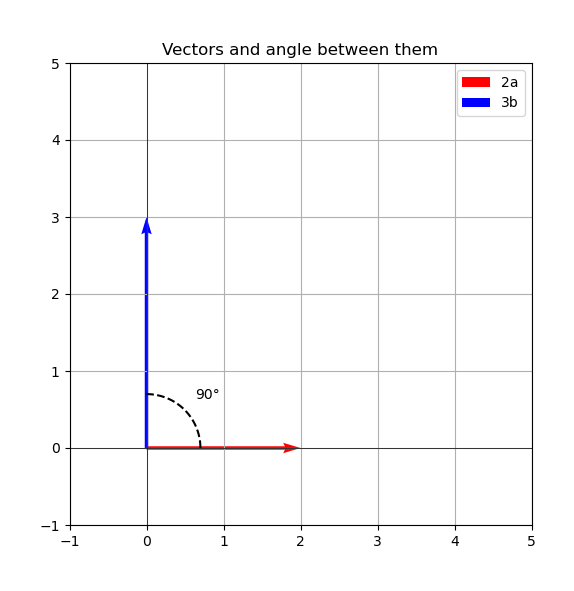
\includegraphics[width=0.8\linewidth]{figs/fig.png}
\end{frame}
% ---------- C CODE ----------
\begin{frame}[fragile]{C Code (code.c)}
\begin{lstlisting}[language=C]
#include<math.h>

double angle_between(double p, double q, double r, double s) {
    double numerator   = - (p*p + q*q - r*r - s*s);
    double denominator = 2.0 * (p*q - r*s);
    double cos_theta   = numerator / denominator;
    return acos(cos_theta);
}
\end{lstlisting}
\end{frame}
\begin{frame}[fragile]{Python Code (code.py)}
\begin{lstlisting}[language=Python]
import numpy as np
import matplotlib.pyplot as plt
import math

if __name__ == "__main__":
    # Define two unit vectors directly
    a = np.array([1, 0])                   # along x-axis
    b = np.array([0, 1])                   # along y-axis (90° from a)

    # Scale them like in the specific case
    a_scaled = 2 * a
    b_scaled = 3 * b
# Compute angle
    dot_product = np.dot(a, b)
\end{lstlisting}
\end{frame}
\begin{frame}[fragile]{Python Code (code.py)}
\begin{lstlisting}[language=Python]
    theta = math.acos(dot_product / (np.linalg.norm(a) * np.linalg.norm(b)))
    print("Angle (radians):", theta)
    print("Angle (degrees):", math.degrees(theta))
    plt.figure(figsize=(6,6))
    ax = plt.gca()
    ax.set_aspect('equal')
    # Plot vectors
    plt.quiver(0, 0, a_scaled[0], a_scaled[1], angles='xy', scale_units='xy', scale=1,
               color='r', label='2a')
    plt.quiver(0, 0, b_scaled[0], b_scaled[1], angles='xy', scale_units='xy', scale=1,
               color='b', label='3b')
\end{lstlisting}
\end{frame}
\begin{frame}[fragile]{Python Code (code.py)}
\begin{lstlisting}[language=Python]
    angle_arc = np.linspace(0, theta, 100)
    plt.plot(0.7*np.cos(angle_arc), 0.7*np.sin(angle_arc), 'k--')
    plt.text(0.9*math.cos(theta/2), 0.9*math.sin(theta/2), f"{math.degrees(theta):.0f}°")
    plt.axhline(0, color='black', linewidth=0.5)
    plt.axvline(0, color='black', linewidth=0.5)
    plt.xlim(-1, 5)
    plt.ylim(-1, 5)
    plt.legend()
    plt.title("Vectors and angle between them (Python only)")
    plt.grid(True)
    plt.show()
\end{lstlisting}
\end{frame}
\begin{frame}[fragile]{Python Code (nativecode.py)}
\begin{lstlisting}[language=Python]
from ctypes import CDLL, c_double
import os, math
import numpy as np
import matplotlib.pyplot as plt

# Load the shared library (libcode.so must be in the same folder)
_lib_path = os.path.join(os.path.dirname(__file__), "code.so")
_lib = CDLL(_lib_path)

# Define arg and return types
_lib.angle_between.argtypes = [c_double, c_double, c_double, c_double]
_lib.angle_between.restype  = c_double
\end{lstlisting}
\end{frame}
\begin{frame}[fragile]{Python Code (nativecode.py)}
\begin{lstlisting}[language=Python]
def angle_between(p, q, r, s):
    """Call the C function and return angle in radians"""
    return _lib.angle_between(p, q, r, s)

if __name__ == "__main__":
    # Specific case: p=2, q=3, r=3, s=-2
    p, q, r, s = 2, 3, 3, -2
    theta = angle_between(p, q, r, s)
    print("Angle (radians):", theta)
    print("Angle (degrees):", math.degrees(theta))

    # Pick two unit vectors with the computed angle
    # Take a = (1,0), then b = (cosθ, sinθ)
\end{lstlisting}
\end{frame}
\begin{frame}[fragile]{Python Code (nativecode.py)}
\begin{lstlisting}[language=Python]
    a = np.array([1, 0])
    b = np.array([math.cos(theta), math.sin(theta)])

    # Scale them for visualization
    a_scaled = p * a
    b_scaled = q * b

    plt.figure(figsize=(6,6))
    ax = plt.gca()
    ax.set_aspect('equal')

\end{lstlisting}
\end{frame}
\begin{frame}[fragile]{Python Code (nativecode.py)}
\begin{lstlisting}[language=Python]
# Plot vectors
    plt.quiver(0, 0, a_scaled[0], a_scaled[1], angles='xy', scale_units='xy', scale=1,
               color='r', label='2a')
    plt.quiver(0, 0, b_scaled[0], b_scaled[1], angles='xy', scale_units='xy', scale=1,
               color='b', label='3b')

    # Draw angle arc
    angle_arc = np.linspace(0, theta, 100)
    plt.plot(0.7*np.cos(angle_arc), 0.7*np.sin(angle_arc), 'k--')
    plt.text(0.9*math.cos(theta/2), 0.9*math.sin(theta/2), f"{math.degrees(theta):.0f}°")
\end{lstlisting}
\end{frame}
\begin{frame}[fragile]{Python Code (nativecode.py)}
\begin{lstlisting}[language=Python]
    # Axes
    plt.axhline(0, color='black', linewidth=0.5)
    plt.axvline(0, color='black', linewidth=0.5)
    plt.xlim(-1, max(p,q)+2)
    plt.ylim(-1, max(p,q)+2)
    plt.legend()
    plt.title("Vectors and angle between them")
    plt.grid(True)
    plt.show()
\end{lstlisting}
\end{frame}
\end{document}